% Created 2017-05-14 Sun 11:57
% Intended LaTeX compiler: pdflatex
\documentclass[presentation,10pt]{beamer}
\usepackage[utf8]{inputenc}
\usepackage[T1]{fontenc}
\usepackage{graphicx}
\usepackage{grffile}
\usepackage{longtable}
\usepackage{wrapfig}
\usepackage{rotating}
\usepackage[normalem]{ulem}
\usepackage{amsmath}
\usepackage{textcomp}
\usepackage{amssymb}
\usepackage{capt-of}
\usepackage{hyperref}
\usepackage{amsthm}
\usepackage{amsmath}
\usepackage{mathtools}
\newtheorem{mydef}{Definition}
\newtheorem{mythm}{Theorem}
\newcommand{\dx}{\mathrm{d}}
\newcommand{\var}{\mathrm{var}}
\newcommand{\cov}{\mathrm{cov}}
\newcommand{\corr}{\mathrm{corr}}
\newcommand{\pr}{\mathrm{Pr}}
\newcommand{\rarrowd}[1]{\xrightarrow{\text{ \textit #1 }}}
\DeclareMathOperator*{\plim}{plim}
\newcommand{\plimn}{\plim_{n \rightarrow \infty}}
\usepackage{booktabs}
\usepackage{color}
\setlength{\parskip}{1em}
\usetheme{CambridgeUS}
\usecolortheme{beaver}
\author{Zheng Tian}
\date{}
\title{Lecture 10: Nonlinear Regression Functions}
\hypersetup{
 pdfauthor={Zheng Tian},
 pdftitle={Lecture 10: Nonlinear Regression Functions},
 pdfkeywords={},
 pdfsubject={},
 pdfcreator={Emacs 25.1.1 (Org mode 9.0.3)}, 
 pdflang={English}}
\begin{document}

\maketitle
\begin{frame}{Outline}
\setcounter{tocdepth}{1}
\tableofcontents
\end{frame}



\section{Introduction}
\label{sec:org961cdda}

\begin{frame}[label={sec:orge630e1b}]{Overview}
\begin{block}{Linear population regression function}
\(E(Y_i \mid \mathbf{X}_i) = \beta_0 + \beta_1 X_{i1} + \cdots + \beta_k
X_{ik}\), where \(\mathbf{X}_i = (X_{i1}, \ldots, X_{ik})^{\prime}\). 
\end{block}

\begin{block}{Nonlinear population regression function}
\(E(Y_i \mid \mathbf{X}_i) = f(X_{i1}, X_{i2}, \ldots, X_{ik};
\beta_1, \beta_2, \ldots, \beta_m)\), where \(f(\cdot)\) is a nonlinear function.
\end{block}

\begin{block}{Study questions}
\begin{itemize}
\item Why do we need to use nonlinear regression models?
\item What types of nonlinear regression models can we estimate by OLS?
\item How can we interpret the coefficients in nonlinear regression models?
\end{itemize}
\end{block}
\end{frame}

\section{A General Strategy For Modeling Nonlinear Regression Functions}
\label{sec:orgff5816b}

\begin{frame}[label={sec:org199bf40}]{Test Scores and district income}
\begin{columns}
\begin{column}{0.4\columnwidth}
\begin{itemize}
\item Test scores can be determined by average district income

\item We estimate a simple linear regression model
\[TestScore = \beta_0 + \beta_1 Income + u\]

\item What's the problem with the simple linear regression model?
\end{itemize}
\end{column}
\begin{column}{0.6\columnwidth}
\begin{figure}[htbp]
\centering
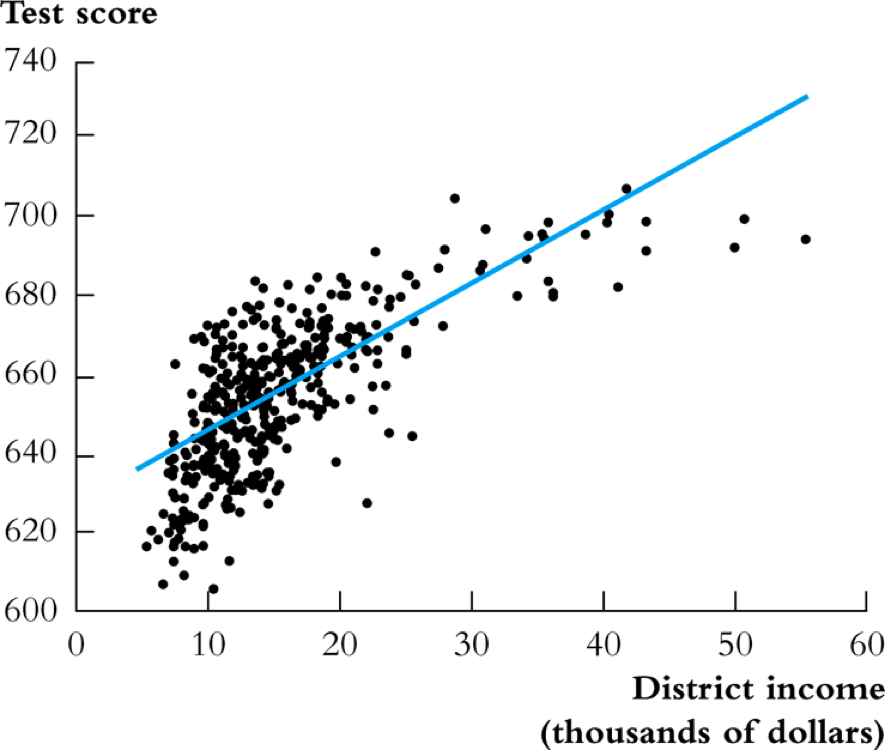
\includegraphics[width=0.85\textwidth]{img/fig-8-2.png}
\caption{\label{fig:org56281dc}
Scatterplot of test score vs district income and a linear regression line}
\end{figure}
\end{column}
\end{columns}
\end{frame}

\begin{frame}[label={sec:org40cabb1}]{Why does a simple linear regression model not fit the data well?}
\begin{itemize}
\item Data points are below the OLS line when income is very low (under
\$10,000) or very high (over \$40,000), and are above the line when
income is between \$15,000 and \$30,000.

\vspace{0.1cm}
\item The scatterplot may imply a curvature in the relationship between
test scores and income. 

\vspace{0.1cm}
That is, a unit increase in income may have larger effect on test
scores when income is very low than when income is very high.

\vspace{0.1cm}
\item The linear regression line cannot capture the curvature because the
effect of district income on test scores is constant over all the
range of income since 
\[\Delta TestScore / \Delta Income = \beta_1\]
where \(\beta_1\) is constant.
\end{itemize}
\end{frame}

\begin{frame}[label={sec:orgc9d8c89}]{Estimate a quadratic regression model}
\begin{equation}
\label{eq:quadratic-testscore}
TestScore = \beta_0 + \beta_1 Income + \beta_2 Income^2 + u
\end{equation}

\begin{itemize}
\item This model is nonlinear, specifically quadratic, with respect to
\(Income\) since we include the squared income.

\item The population regression function is
\[E(TestScore | Income) = \beta_0 + \beta_1 Income + \beta_2 Income^2\]

\item It is linear with respect to \(\beta\). So we can still use the
OLS estimation and carry out hypothesis testing as we do with a
linear regression model.
\end{itemize}
\end{frame}

\begin{frame}[label={sec:org27a43d4}]{Estimate a quadratic regression model (cont'd)}
\begin{figure}[htbp]
\centering
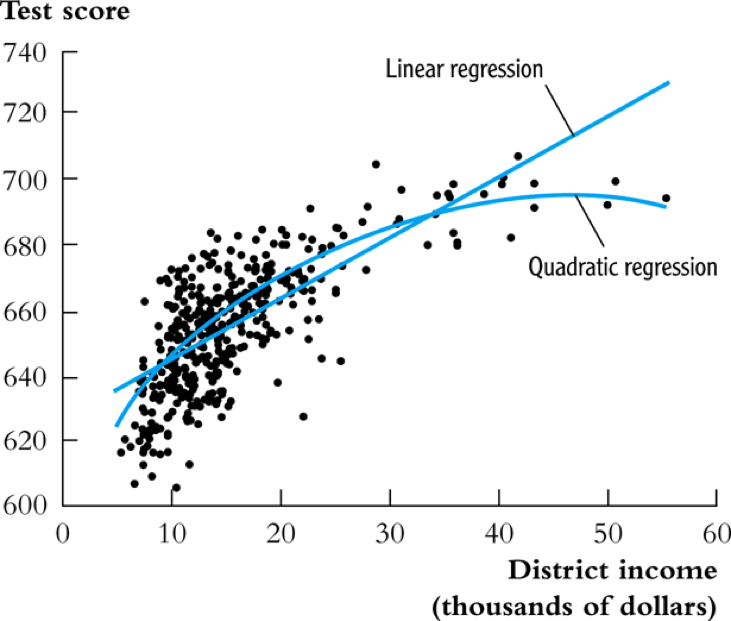
\includegraphics[width=0.6\textwidth,height=0.5\textwidth]{img/fig-8-3.png}
\caption{\label{fig:org14b951b}
Scatterplot of test score vs district income and a quadratic regression line}
\end{figure}
\end{frame}

\begin{frame}[shrink,label={sec:org2f0a066}]{A general formula for a nonlinear population regression function}
A general nonlinear regression model is

\begin{equation}
\label{eq:nl-general}
Y_i = f(X_{i1}, X_{i2}, \ldots, X_{ik}; \beta_1, \beta_2, \ldots, \beta_m) + u_i
\end{equation}

\begin{itemize}
\item The \alert{population nonlinear regression function}: 
\[ E(Y_i | X_{i1}, \ldots, X_{ik}) = f(X_{i1}, X_{2i}, \ldots, X_{ik}; \beta_1, \beta_2, \ldots, \beta_m) \]
\item The number of regressors and the number of parameters are not
necessarily equal in the nonlinear regression model.
\item In vector notation 
\begin{equation}
\label{eq:nl-general-mat}
Y_i = f(\mathbf{X}_i; \boldsymbol{\beta}) + u_i
\end{equation}
\item We focus on the nonlinear regression models
such that \(f(\cdot)\) is \alert{nonlinear with \(\mathbf{X}_i\)} but \alert{linear with
\(\boldsymbol{\beta}\)}.
\end{itemize}
\end{frame}

\begin{frame}[label={sec:orgf0d445a}]{The effect on \(Y\) of a change in a regressor}
\begin{block}{For any general nonlinear regression function}
The effect on \(Y\) of a change in one regressor, say \(X_1\), holding
other things constant, can be computed as
\begin{equation}
\label{eq:nl-gen-effect}
\Delta Y = f(X_1 + \Delta X_1, X_2, \ldots, X_k; \boldsymbol{\beta}) - f(X_1, X_2, \ldots, X_k; \boldsymbol{\beta})
\end{equation}
\end{block}

\begin{block}{For continuous and differentiable nonlinear functions}
When \(X_1\) and \(Y\) are continuous variables and \(f(\cdot)\) is
differentiable, the marginal effect of \(X_1\) is the partial derivative
of \(f\) with respect to \(X_1\), that is, holding other things constant
\[ \mathrm{d}Y = \frac{\partial f(X_1, \ldots, X_k;
\boldsymbol{\beta})}{\partial X_i} \mathrm{d} X_i \]
because \(\mathrm{d}X_j = 0\) for \(j \neq i\)
\end{block}
\end{frame}

\begin{frame}[label={sec:org3875435}]{Application to test scores and income}
\begin{block}{Estimation}
\begin{equation}
\label{eq:tsr-income2}
\widehat{TestScore} = \underset{\displaystyle (2.9)}{607.3} +
\underset{\displaystyle (0.27)}{3.85}Income - \underset{\displaystyle (0.0048)}{0.0423}Income^2,\, \bar{R}^2 = 0.554
\end{equation}
\end{block}

\begin{block}{Hypothesis test}
Test \(H_0:\, \beta_2 = 0 \text{ vs. } H_1:\,\beta_2 \neq 0\). 
\[ t = \frac{-0.0423}{0.0048} = -8.81 > -1.96 \]
We reject the null at the 1\%, 5\% and 10\% significance levels, and
therefore, confirm the quadratic relationship between test scores
and income. 
\end{block}
\end{frame}

\begin{frame}[label={sec:org81f64fa}]{The effect of change in income on test scores}
\begin{block}{A change in income from \$10 thousand to \$20 thousand}
\begin{equation*}
\begin{split}
\Delta \hat{Y} &= \hat{\beta}_0 + \hat{\beta}_1 \times 11 + \hat{\beta}_2 \times 11^2 - (\hat{\beta}_0 + \hat{\beta}_1 \times 10 + \hat{\beta}_2 \times 10^2) \\
&= \hat{\beta}_1 (11 - 10) + \hat{\beta}_2(11^2 - 10^2) \\
& = 3.85 - 0.0423 \times 21 = 2.96
\end{split}
\end{equation*}
\end{block}

\begin{block}{A change in income from \$40 thousand to \$41 thousand}
\begin{equation*}
\begin{split}
\Delta \hat{Y} &= \hat{\beta}_0 + \hat{\beta}_1 \times 41 + \hat{\beta}_2 \times 41^2 - (\hat{\beta}_0 + \hat{\beta}_1 \times 40 + \hat{\beta}_2 \times 40^2) \\
&= \hat{\beta}_1 (41 - 40) + \hat{\beta}_2(41^2 - 40^2) \\
& = 3.85 - 0.0423 \times 81 = 0.42
\end{split}
\end{equation*}
\end{block}
\end{frame}

\begin{frame}[label={sec:orgb3da4ed}]{A general approach to modeling nonlinearities using multiple regression}
\begin{enumerate}
\item Identify a possible nonlinear relationship.
\begin{itemize}
\item Economic theory
\item Scatterplots
\item Your judgment and experts' opinions
\end{itemize}

\item Specify a nonlinear function and estimate its parameters by OLS.
\begin{itemize}
\item The OLS estimation and inference techniques can be used as usual
when the regression function is linear with respect to \(\beta\).
\end{itemize}

\item Determine whether the nonlinear model can improve a linear model
\begin{itemize}
\item Use t- and/or F-statistics to test the null hypothesis that the
population regression function is linear against the alternative
that it is nonlinear.
\end{itemize}

\item Plot the estimated nonlinear regression function.

\item Compute the effect on \emph{Y} of a change in \emph{X} and interpret the results.
\end{enumerate}
\end{frame}


\section{Nonlinear functions of a single independent variable}
\label{sec:org5696b1e}

\begin{frame}[label={sec:org8db2e0b}]{Polynomials}
\begin{block}{A polynomial regression model of degree r}
\begin{equation}
\label{eq:poly-r}
Y_i = \beta_0 + \beta_1 X_i + \beta_2 X_i^2 + \cdots + \beta_r X_i^r + u_i
\end{equation}
\begin{itemize}
\item \(r = 2\): a \alert{quadratic} regression model
\item \(r = 3\): a \alert{cubic} regression model
\item Use the OLS method to estimate \(\beta_1, \beta_2, \ldots, \beta_r\).
\end{itemize}
\end{block}

\begin{block}{Testing the null hypothesis that the population regression function is linear}
\[ H_0:\, \beta_2 = 0, \beta_3 = 0, ..., \beta_r = 0 \text{ vs. }
H_1:\, \text{ at least one } \beta_j \neq 0, j = 2, \ldots, r \]

Use F statistic to test this joint hypothesis. The number of
restriction is \(q = r-1\).
\end{block}
\end{frame}

\begin{frame}[label={sec:org913a5cc}]{What is \(\Delta Y / \Delta X\) in a polynomial regression model?}
\begin{itemize}
\item Consider a cubic model and continuous \(X\) and \(Y\)
\[Y = \beta_0 + \beta_1 X + \beta_2 X^2 + \beta_3 X^3 + u\]

\item Then, we can calculate
\[\frac{\dx Y}{\dx X} = \beta_1 + 2\beta_2 X + 3\beta_3 X^2 \]

\item The effect of a unit change in \(X\) on \(Y\) depends on the value of
\(X\) at evaluation.
\end{itemize}
\end{frame}

\begin{frame}[label={sec:orgcdc9262}]{Which degree of polynomial should I use?}
\begin{itemize}
\item Balance a trade-off between flexibility and statistical precision.
\begin{itemize}
\item Flexibility. Relate Y to X in more complicated way than simple
linear regression.
\item Statistical precision. \(X, X^2, X^3, \ldots\) are correlated so
that there is the problem of imperfect multicollinearity.
\end{itemize}
\item Follow a sequential hypothesis testing procedure
\begin{enumerate}
\item Pick a maximum value of \(r\) and estimate the polynomial
regression for that \(r\).
\item Follow a "deletion" rule based on t-statistic or F-statistic.
\end{enumerate}
\end{itemize}
\end{frame}

\begin{frame}[shrink,label={sec:orgb6413a9}]{Application to district income and test scores}
We estimate a cubic regression model relating test scores to district
income as follows
\begin{equation*}
\widehat{TestScore} = \underset{\displaystyle (5.1)}{600.1} 
                    + \underset{\displaystyle (0.71)}{5.02} Income
                    - \underset{\displaystyle (0.029)}{0.096} Income^2 
                    + \underset{\displaystyle (0.00035)}{0.00069} Income^3, \hat{R}^2 = 0.555 
\end{equation*}

\begin{block}{Test whether it is a cubic model}
The t-statistic for \(H_0: \beta_3 = 0\) is 1.97 \(\Rightarrow\) Fail to reject
\end{block}

\begin{block}{Test whether it is a nonlinear model}
The F-statistic for \(H_0: \beta_2 = \beta_3 = 0\) is 37.7, p-value
\(<0.01\)
\end{block}

\begin{block}{Interpretation of coefficients}
Use the general formula of interpreting the effect of \(\Delta X\) on
\(Y\).
\end{block}
\end{frame}

\begin{frame}[label={sec:orgb081826}]{A natural logarithmic function \(y = \ln(x)\)}
\begin{itemize}
\item Properties of \(\ln(x)\)
\begin{gather*}
\ln(1/x) = -\ln(x),\, \ln(ax) = \ln(a) + \ln(x) \\
\ln(x/a) = \ln(x) - \ln(a),\, \text{ and } \ln(x^a) = a\ln(x)
\end{gather*}

\item The derivative of \(\ln(x)\) is
\[ \frac{\dx \ln(x)}{\dx x} = \lim_{\Delta x \rightarrow 0}
  \frac{\ln(x + \Delta x) - \ln(x)}{\Delta x} = \frac{1}{x}\,\text{.} \]
It follows that \(\dx \ln(x) = \dx x / x\), representing the percentage
change in \(x\).
\end{itemize}
\end{frame}

\begin{frame}[label={sec:org58b2517}]{The percentage-change form using \(\ln(x)\)}
\begin{itemize}
\item The change in \(\ln(X)\) represents the percentage change in \(X\)

\[ \ln(x + \Delta x) - \ln(x) \approx \frac{\Delta x}{x} \text{ when
  } \Delta x \text{ is small.} \]

\item The Taylor expansion of \(\ln(x +
  \Delta x)\) at \(x\), which is
\begin{align*}
\ln(x + \Delta x) &= \ln(x) + \frac{\dx \ln(x)}{\dx x} (x + \Delta x - x) + \frac{1}{2!}\frac{\dx^2 \ln(x)}{\dx x^2}(x + \Delta x - x)^2 + \cdots \\
                  &= \ln(x) + \frac{\Delta x}{x} -\frac{\Delta x^2}{2x^2} + \cdots
\end{align*}
When \(\Delta x\) is very small, we can omit the terms with \(\Delta
  x^2, \Delta x^3\), etc. Thus, we have \(\ln(x + \Delta x) - \ln(x)
  \approx \frac{\Delta x}{x}\) when \(\Delta x\) is small.
\end{itemize}
\end{frame}

\begin{frame}[label={sec:org901361e}]{The three logarithmic regression models}
There are three types of logarithmic regression models:

\begin{itemize}
\item Linear-log model

\item Log-linear model

\item Log-log model
\end{itemize}

Differences in logarithmic transformation of \(X\) and/or \(Y\) lead to
differences in interpretation of the coefficient.
\end{frame}

\begin{frame}[label={sec:org5db1ae3}]{Case I: linear-log model}
\begin{itemize}
\item \alert{Model form}. \(X\) is in logarithms, \(Y\) is not.
\begin{equation}
\label{eq:linear-log}
Y_i = \beta_0 + \beta_1 \ln(X_i) + u_i, i = 1, \ldots, n
\end{equation}

\item \alert{Interpretation}. a 1\% change in \(X\) is associated with a
change in \(Y\) of 0.01\(\beta_{\text{1}}\)
\[ \Delta Y = \beta_1 \ln(X + \Delta X) - \beta_1 \ln(X) \approx
  \beta_1 \frac{\Delta X}{X} \]

\item \alert{Example}. The estimated model is 
\[\widehat{TestScore} = 557.8 + 36.42\ln(Income)\] 
\begin{itemize}
\item 1\% increase in average district income results in an increase in
test scores by \(0.01 \times 36.42 = 0.36\) point.
\end{itemize}
\end{itemize}
\end{frame}

\begin{frame}[label={sec:orge5c3e3c}]{Case II: log-linear model}
\begin{itemize}
\item \alert{Model form}. \(Y\) is in logarithms, \(X\) is not.
\begin{equation}
\label{eq:log-linear}
\ln(Y_i) = \beta_0 + \beta_1 X_i + u_i
\end{equation}

\item \alert{Interpretation}. A one-unit change in \(X\)
is associated with a \(100 \times \beta_1\%\) change in \(Y\) because
\begin{equation*}
\frac{\Delta Y}{Y} \approx \ln(Y + \Delta Y) - \ln(Y) = \beta_1 \Delta X
\end{equation*}

\item \alert{Example}. 
\[ \widehat{\ln(Earnings)} = 2.805 + 0.0087Age \]
\begin{itemize}
\item Earnings are predicted to increase by 0.87\% for each additional
year of age.
\end{itemize}
\end{itemize}
\end{frame}

\begin{frame}[shrink,label={sec:orgf8c8a05}]{Case III: log-log model}
\begin{itemize}
\item \alert{Model form}. Both \(X\) and \(Y\) are in logarithms.
\begin{equation}
\label{eq:log-log}
\ln(Y_i) = \beta_0 + \beta_1 \ln(X_i) + u_i
\end{equation}

\item \alert{Interpretation: elasticity}. 1\% change in \(X\) is associated with a
\(\beta_{\text{1}}\)\% change in \(Y\) because 
\begin{equation*}
\frac{\Delta Y}{Y} \approx \ln(Y +
\Delta Y) - \ln(Y) = \beta_1 (\ln(X + \Delta X) - \ln(X)) \approx
\beta_1 \frac{\Delta X}{X}
\end{equation*}

\begin{itemize}
\item \(\beta_{\text{1}}\) is the \alert{elasticity} of \(Y\) with respect to \(X\), that is 
\[ \beta_1 = \frac{100 \times
    (\Delta Y / Y)}{100\times (\Delta X / X)} =\frac{\text{percentage
    change in } Y}{\text{percentage change in } X} \]
\item With the derivative, \(\beta_1 = \dx \ln(Y) / \dx \ln(X) = (\dx Y/Y)
    / (\dx X/X)\).
\end{itemize}

\item \alert{Example}. The log-log model of the test score application is
estimated as
\[ \widehat{\ln(TestScore)} = 6.336 + 0.0544 \ln(Income) \]
This implies that a 1\% increase in income corresponds to a
0.0544\% increase in test scores.
\end{itemize}
\end{frame}

\begin{frame}[label={sec:org8b6d19c}]{The log-linear and log-log regression functions}
\begin{figure}[htbp]
\centering
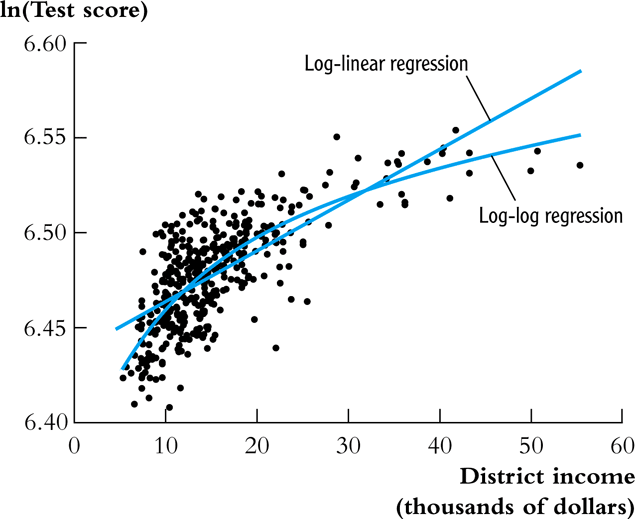
\includegraphics[width=0.65\textwidth]{img/fig-8-6.png}
\caption{\label{fig:org0f76a56}
The log-linear and log-log regression functions}
\end{figure}
\end{frame}

\begin{frame}[label={sec:orgcb0cfe5}]{Summary}
\begin{center}
\begin{tabular}{p{4cm}p{6cm}}
Regression specification & Interpretation of \(\beta_1\)\\
\hline
\(Y = \beta_0 + \beta_1 \ln(X) + u\) & A 1\% change in X is associated with a change in Y of \(0.01\beta_{1}\)\\
\hline
\(\ln(Y) = \beta_0 + \beta_1 X + u\) & A change in X by one unit is associated with a \(100\beta_1\%\) change in Y\\
\hline
\(\ln(Y) = \beta_0 + \beta_1 \ln(X) + u\) & A 1\% change in X is associated with a \(\beta_{1}\%\) change in Y, so \(\beta_1\) is the elasticity of Y with respect to X\\
\end{tabular}
\end{center}
\end{frame}
\end{document}